\section{Construction of Green's Functions by Orthonormal Series Expansion}
\subsection{Systems of Orthonormal Functions}
\begin{itemize}
        \item General form of the orthogonality relation (normalized):
\begin{equation*}
  \int\limits_{a}^{b}U_{m}(x)U_{n}^{*}(x)\,\mathrm{d}x = \delta_{mn}
\end{equation*}
  \item Completeness relation
        \begin{equation*}
          \sum\limits_{n=1}^{\infty} U_{n}(x)\,U^{*}_{n}(x') = \delta(x - x')
        \end{equation*}
  \item Always valid for certain function spaces, e.g. even, odd
        \begin{align*}
          \delta(x - x') = \dfrac{2}{d} \sum\limits_{n=1}^{\infty}
          \left[
          \sin\left(\dfrac{\pi n}{d}\right)
          \,
          \sin\left(\dfrac{\pi n}{d}\right)
          \right]
        \end{align*}
\end{itemize}
\subsection{Constructing a Green's Function for the Domain Outside of a Wedge (2D Problem)}
\begin{align*}
  &\Delta_{2}G_{D}(\bs{r}, \bs{r'}) = - \delta (\bs{r} - \bs{r'}),\\
  &G_{D}(\bs{r}, \bs{r'}) = 0\text{ for } \varphi=0 \lor \varphi=\alpha
\end{align*}
\begin{center}
  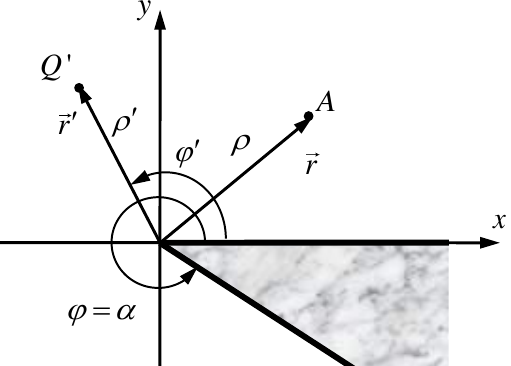
\includegraphics[width=.3\paperheight]{content/caem/pictures/conducting_wedge.png}
\end{center}
\begin{enumerate}
  \item Formulation in cylindrical coordinates:
        \begin{align*}
          &\dfrac{1}{\rho} \dfrac{\partial}{\partial\rho}\left(\rho \dfrac{\partial}{\partial\rho}G\right)
          + \dfrac{1}{\rho^{2}}\dfrac{\partial^{2}}{\partial \varphi^{2}}G\\
          = &-\dfrac{1}{\rho} \delta(\rho - \rho') \delta(\varphi - \varphi')
        \end{align*}
  \item Seperation ansatz for homogeneous problem:
        \begin{align*}
          &\phi(\rho, \varphi) = h(\rho) f(\varphi),\\
          &\underbrace{\dfrac{\rho}{h(\rho)} \dfrac{\partial}{\partial\rho} \left[\rho \dfrac{\partial}{\partial\rho} h(\rho)\right]}_{\nu^{2}}
            + \underbrace{\dfrac{1}{f(\varphi)} \dfrac{\partial^{2}}{\partial\varphi^{2}} f(\varphi)}_{-\nu^{2}}
            = 0\\
          & \dfrac{\partial^{2}}{\partial\varphi^{2}}f(\varphi) + \nu^{2}f(\varphi) = 0
            \implies f(\varphi) \text{\texttildelow} \left\{e^{\pm j\nu \varphi}\right\}
          \begin{Bmatrix} \sin(\nu\varphi)\\ \cos(\nu\varphi) \end{Bmatrix}\\
          & \dfrac{\partial}{\partial\rho} \left[\rho \dfrac{\partial}{\partial\rho} h(\rho)\right] - \nu^{2}\dfrac{h(\rho)}{\rho} = 0
            \implies h(\rho) \, \text{\texttildelow} \, \rho^{\nu}, \rho^{-\nu}
        \end{align*}
  \item Ansatz for $G_{D}$ (fulfills BC in $\varphi$ and symmetry in $\varphi, \varphi'$)
        \begin{equation*}
          G_{D}(\rho, \varphi, \rho', \varphi') = \sum\limits_{n=1}^{\infty} g_{n}(\rho, \rho')
          \dfrac{2}{\alpha}
          \sin\left(\dfrac{n\pi}{\alpha} \varphi\right)
          \sin\left(\dfrac{n\pi}{\alpha} \varphi'\right)
        \end{equation*}
  \item Solution after reducing problem to 1D and solving coefficients using the ``jump'' equation:
        \begin{align*}
          &G_{D}(\rho, \varphi, \rho', \varphi')\\
          = &\dfrac{1}\pi \sum\limits_{n=1}^{\infty} \dfrac{1}{n}
          \sin\left(\dfrac{n\pi}{\alpha} \varphi\right)
          \sin\left(\dfrac{n\pi}{\alpha} \varphi'\right)
          \rho_{<}^{\frac{n\pi}{\alpha}}
          \rho_{>}^{-\frac{n\pi}{\alpha}}
        \end{align*}
\end{enumerate}
\subsection{Linearly Independant Solutions of the Laplace Equation in Spherical Coordinates}
\subsection{Constructing Green's functions in 2 or 3 dimensions by reducing to 1D problem}
\begin{enumerate}
  \item Express the problem $\mathcal{L}\{G(\bs{r}-\bs{r'})\} = -\delta(\bs{r}-\bs{r'})$ in an appropriate coordinate system for the boundary conditions.
        \begin{equation*}
          \mathcal{L}\left\{G(q_{1}, q_{2}, q_{3})\right\} = -\delta(q_{1}-q_{1}') \delta(q_{2}-q_{2}') \delta(q_{3}-q_{3}')
        \end{equation*}
  \item Find solutions to the homogeneous problems (eigenfunctions corresponding to operator):
        \begin{align*}
          \mathcal{\hat{L}} \left\{U(q_{1})\right\} = c_{1}U(q_{1}) & & U_{m}(q_{1})\\
          \mathcal{\tilde{L}} \left\{V(q_{2})\right\} = c_{2}V(q_{2}) & \implies & V_{n}(q_{2})\\
          \mathcal{\bar{L}} \left\{W(q_{3})\right\} = c_{3}W(q_{3}) & & W_{l}(q_{3})
        \end{align*}
  \item Reduce to new 1D problem using \textbf{completeness} (term by term equality) and \textbf{orthogonality} in one or two coordinates:
        \begin{align*}
          &G = \sum\limits_{n} g_{n}(q_{3},q'_{3}) U_{n}(q_{1},q_{2})U_{n}(q'_{1},q'_{2})\\
          &\sum\limits_{n} U_{n}(q_{1},q_{2}) U_{n}(q'_{1},q'_{2}) = \delta(q_{1}-q'_{1})\delta(q_{2}-q'_{2})\\
          &\implies \mathcal{L'}\left\{g_{n}(q_{3},q'_{3})\right\} = -\delta(q_{3}-q'_{3})
        \end{align*}
  \item Find 1D Green's function for the new 1D problem
        \begin{equation*}
          \mathcal{L'}\left\{g_{n}(q_{3},q'_{3})\right\} = -\delta(q_{3}-q'_{3})
        \end{equation*}
\end{enumerate}

\subsection{Systematic procedure for a Green's function of 2nd order ordinary differential operator}
\begin{itemize}
  \item Use two linearly independant solutions $f_1$ and $f_2$ of homogeneous problem \(\mathcal{L}\{f_{1/2}(x)\} = 0\)
  \item Generate particular solutions on both sides of the source location
        \begin{align*}
          u_{1}(x) = A_{1} f_{1}(x) + A_{2} f_{2}(x), \quad x < x'\\
          u_{1}(x) = B_{1} f_{1}(x) + B_{2} f_{2}(x), \quad x > x'\\
        \end{align*}
  \item Choose a Green's function of the form
        \begin{equation*}
          g(x, x') = h \, u_{1}(x_{<})u_{2}(x_{>})
        \end{equation*}
  \item Determine the constant h according to
        \begin{equation*}
          h = \dfrac{-1}{\mathcal{W}\{u_{1}(x), u_{2}(x)\}}
        \end{equation*}
        whereas $\mathcal{W}\{\cdot\}$ is the Wronski determinant (``Jump'' equation is automatically fulfilled). $\mathcal{W}\{\cdot\}$ can either be calculated or looked up in textbooks such as \textit{Handbook of Mathematics} by \textsc{Abramowitz and Stegun}.
\end{itemize}

\begin{definition}{Wronski Determinant}
  \todo{Add definition here}
  \begin{equation*}
    \mathcal{W}\{f_{1}, f_{2}\} = f_{1}\cdot f_{2}' - f_{1}'\cdot f_{2},
  \end{equation*}
  and for linear combinations we get:
  \begin{equation*}
    \mathcal{W}\{u_{1}, u_{2}\} = (A_{1}B_{2} - A_{2}B_{1}) \cdot \mathcal{W}\{f_{1}, f_{2}\},
  \end{equation*}
  \begin{align*}
    &u_{1}(x) = A_{1}f_{1}(x) + A_{2}f_{2}(x),\\
    &u_{2}(x) = B_{1}f_{1}(x) + B_{2}f_{2}(x).
  \end{align*}
\end{definition}

\begin{info}{Wronski determinants of Bessel (Hankel) functions}
  \begin{tabular}{>{$}l<{$}>{$}l<{$}}
    \mathcal{W}\{J_{\nu}, J_{-\nu}\} &= -\dfrac{2}{\pi x} \sin(\nu x)\\\\
    \mathcal{W}\{J_{\nu}, N_{\nu}\} &= \dfrac{2}{\pi x}\\\\
    \mathcal{W}\{H_{\nu}^{(1)}, H_{\nu}^{(2)}\} &= -\dfrac{4j}{\pi x}\\\\
    \mathcal{W}\{J_{\nu}, H_{\nu}^{(1),(2)}\} &= \pm \dfrac{2j}{\pi x}\\\\
    \mathcal{W}\{I_{\nu}, I_{-\nu}\} &= -\dfrac{2}{\pi x} \sin(\nu x)\\\\
    \mathcal{W}\{I_{\nu}, K_{\nu}\} &= -\dfrac{1}{x}\\\\
  \end{tabular}
\end{info}
